\documentclass[10pt]{article}
\usepackage[polish]{babel}
\usepackage[utf8]{inputenc}
\usepackage[T1]{fontenc}
\usepackage{amsmath}
\usepackage{amsfonts}
\usepackage{amssymb}
\usepackage[version=4]{mhchem}
\usepackage{stmaryrd}
\usepackage{graphicx}
\usepackage[export]{adjustbox}
\graphicspath{ {./images/} }

\title{LIGA MATEMATYCZNA im. Zdzisława Matuskiego GRUDZIEŃ 2018 \\
 GIMNAZJUM }

\author{}
\date{}


\begin{document}
\maketitle
(klasa VII i VIII szkoły podstawowej, klasa III gimnazjum)

\section*{ZADANIE 1.}
Liczba \(a\) przy dzieleniu przez 9 daje resztę 2 , a mniejsza od niej liczba \(b\) przy dzieleniu przez 9 daje resztę 7. Znajdź resztę z dzielenia różnicy \(a-b\) przez 9 .

\section*{ZADANIE 2.}
Proste \(p\) i \(q\) są równoległe, a miary kątów przy wierzchołkach \(A\) i \(C\) są równe \(135^{\circ} \mathrm{i} 115^{\circ}\) tak, jak na rysunku. Oblicz miarę kąta \(A B C\).\\
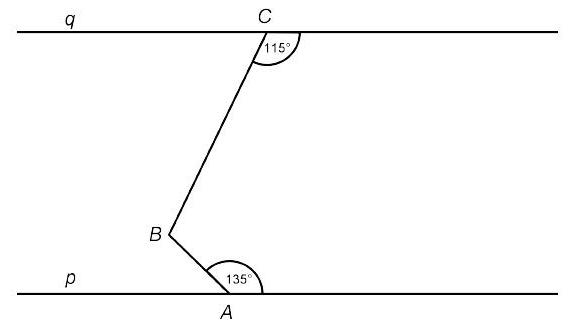
\includegraphics[max width=\textwidth, center]{2024_11_21_aa1016cdd95200a39755g-1(1)}

\section*{ZADANIE 3.}
W wierszu zapisano kolejno 2017 liczb. Pierwsza zapisana liczba jest równa 8, a suma każdych kolejnych siedmiu liczb jest równa 70 . Oblicz ostatnią z zapisanych liczb.

\section*{ZADANIE 4.}
Znajdź takie liczby naturalne \(x, y\), że \(x y=8400 \operatorname{oraz} \operatorname{NWD}\{x, y\}=20\).

\section*{ZADANIE 5.}
Kwadrat \(A\) ma dwa boki pokrywające się z promieniami okręgu, a kwadrat \(B\) ma dwa wierzchołki leżące na tym samym okręgu oraz częściowo współdzieli bok z \(A\). Wyznacz stosunek pola kwadratu \(A\) do pola kwadratu \(B\).\\
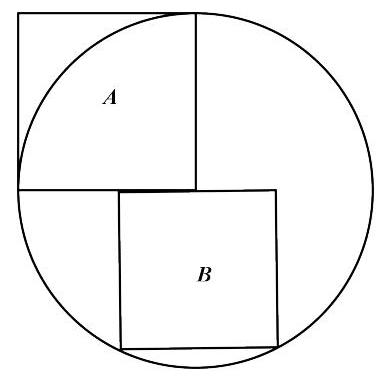
\includegraphics[max width=\textwidth, center]{2024_11_21_aa1016cdd95200a39755g-1}


\end{document}